\documentclass[12pt]{article}

\usepackage{amsthm}
\usepackage{amsmath}
\usepackage{amsfonts}
\usepackage{mathrsfs}
\usepackage{array}
\usepackage{amssymb}
\usepackage{units}
\usepackage{graphicx}
\usepackage{tikz-cd}
\usepackage{nicefrac}
\usepackage{hyperref}
\usepackage{bbm}
\usepackage{color}
\usepackage{tensor}
\usepackage{tipa}
\usepackage{bussproofs}
\usepackage{ stmaryrd }
\usepackage{ textcomp }
\usepackage{leftidx}
\usepackage{afterpage}
\usepackage{varwidth}
\usepackage{tasks}
\usepackage{ cmll }
\usepackage{makecell}
\usepackage{MnSymbol}
\usepackage{multirow}
\usepackage{booktabs}
\usepackage{xparse}
\usepackage{calc}
\usepackage{stackengine}
\usepackage{csquotes}

\newcommand\blankpage{
	\null
	\thispagestyle{empty}
	\addtocounter{page}{-1}
	\newpage
}

\newcommand{\PhantC}{\phantom{\colon}}%
\newcommand{\PhantSQ}{\phantom{\sqrt{\hspace{0.3ex}}}}

% https://tex.stackexchange.com/questions/63355/wrapping-cmidrule-in-a-macro
\ExplSyntaxOn
\makeatletter
\newcommand{\CMidRule}{\noalign\bgroup\@CMidRule{}}
\NewDocumentCommand{\@CMidRule}{
	m % Material to reinsert before cmidrule.
	O{0.0ex} % #1 = left adjust
	O{0.0ex} % #1 = right adjust
	m  %       #3 = columns to span
}{
	\peek_meaning_remove_ignore_spaces:NTF \CMidRule
	{ \@CMidRule { #1 \cmidrule[\cmidrulewidth](l{#2}r{#3}){#4} } }
	{ \egroup #1 \cmidrule[\cmidrulewidth](l{#2}r{#3}){#4} }
}
\makeatother
\ExplSyntaxOff

\graphicspath{ {images/} }

\theoremstyle{plain}
\newtheorem{thm}{Theorem}[subsection] % reset theorem numbering for each chapter
\newtheorem{proposition}[thm]{Proposition}
\newtheorem{lemma}[thm]{Lemma}
\newtheorem{fact}[thm]{Fact}
\newtheorem{cor}[thm]{Corollary}

\theoremstyle{definition}
\newtheorem{defn}[thm]{Definition} % definition numbers are dependent on theorem numbers
\newtheorem{exmp}[thm]{Example} % same for example numbers
\newtheorem{notation}[thm]{Notation}
\newtheorem{remark}[thm]{Remark}
\newtheorem{condition}[thm]{Condition}
\newtheorem{question}[thm]{Question}
\newtheorem{construction}[thm]{Construction}
\newtheorem{exercise}[thm]{Exercise}
\newtheorem{example}[thm]{Example}
\newtheorem{aside}[thm]{Aside}
\newtheorem{algorithm}[thm]{Algorithm}

\def\doubleunderline#1{\underline{\underline{#1}}}
\newcommand{\bb}[1]{\mathbb{#1}}
\newcommand{\scr}[1]{\mathscr{#1}}
\newcommand{\call}[1]{\mathcal{#1}}
\newcommand{\psheaf}{\text{\underline{Set}}^{\scr{C}^{\text{op}}}}
\newcommand{\und}[1]{\underline{\hspace{#1 cm}}}
\newcommand{\adj}[1]{\text{\textopencorner}{#1}\text{\textcorner}}
\newcommand{\comment}[1]{}
\newcommand{\lto}{\longrightarrow}
\newcommand{\rone}{(\operatorname{R}\bold{1})}
\newcommand{\lone}{(\operatorname{L}\bold{1})}
\newcommand{\rimp}{(\operatorname{R} \multimap)}
\newcommand{\limp}{(\operatorname{L} \multimap)}
\newcommand{\rtensor}{(\operatorname{R}\otimes)}
\newcommand{\ltensor}{(\operatorname{L}\otimes)}
\newcommand{\rtrue}{(\operatorname{R}\top)}
\newcommand{\rwith}{(\operatorname{R}\&)}
\newcommand{\lwithleft}{(\operatorname{L}\&)_{\operatorname{left}}}
\newcommand{\lwithright}{(\operatorname{L}\&)_{\operatorname{right}}}
\newcommand{\rplusleft}{(\operatorname{R}\oplus)_{\operatorname{left}}}
\newcommand{\rplusright}{(\operatorname{R}\oplus)_{\operatorname{right}}}
\newcommand{\lplus}{(\operatorname{L}\oplus)}
\newcommand{\prom}{(\operatorname{prom})}
\newcommand{\ctr}{(\operatorname{ctr})}
\newcommand{\der}{(\operatorname{der})}
\newcommand{\weak}{(\operatorname{weak})}
\newcommand{\exi}{(\operatorname{exists})}
\newcommand{\fa}{(\operatorname{for\text{ }all})}
\newcommand{\ex}{(\operatorname{ex})}
\newcommand{\cut}{(\operatorname{cut})}
\newcommand{\ax}{(\operatorname{ax})}
\newcommand{\negation}{\sim}
\newcommand{\true}{\top}
\newcommand{\false}{\bot}
\DeclareRobustCommand{\diamondtimes}{%
	\mathbin{\text{\rotatebox[origin=c]{45}{$\boxplus$}}}%
}
\newcommand{\tagarray}{\mbox{}\refstepcounter{equation}$(\theequation)$}
\newcommand{\startproof}[1]{
	\AxiomC{#1}
	\noLine
	\UnaryInfC{$\vdots$}
}
\newcommand\showdiv[1]{\overline{\smash{)}#1}}
\newcommand{\set}{\operatorname{\underline{Set}}}
\newcommand{\coherence}[2]{#1\text{ }\rotatebox{90}{()}_A\text{ }#2}



\newenvironment{scprooftree}[1]%
{\gdef\scalefactor{#1}\begin{center}\proofSkipAmount \leavevmode}%
	{\scalebox{\scalefactor}{\DisplayProof}\proofSkipAmount \end{center} }

\title{The line is part of a circle}
\author{William Troiani}
\date{\today}

\begin{document}
	\maketitle
\section{Introduction}
A mathematical object of interest $X$ is sometimes a subobject $X \rightarrowtail Y$ where $Y$ has structure which makes reasoning about $X$ simpler. For example, the real open interval $(0,1)$ can be embedded inside the circle $[0,1]/(0 \sim 1)$, which is a compact space although $(0,1)$ is not. Note also that the real numbers $\bb{R}$ can be embedded into the complex numbers $\bb{R} \rightarrowtail \bb{C}$ where $\bb{C}$ is an algebraically closed field and $\bb{R}$ is not. Today, we look at a categorical example of this phenomena, the \emph{Yoneda embedding}.

\section{Equivalences of categories and embeddings}

Recall that a functor $F: \scr{C} \lto \scr{D}$ is \textbf{faithful} if for all pairs of objects $(X,Y)$ in $\scr{C}$ the function
\begin{align*}
	\operatorname{Hom}_{\scr{C}}(X,Y) &\lto \operatorname{Hom}_{\scr{D}}(FX, FY)\\
	f &\longmapsto Ff
	\end{align*}
is injective. Also, if this function is surjective then $F$ is \textbf{full}.

Moreover, if for every object $D \in \scr{D}$ there exists an object $C \in \scr{C}$ such that $FC \cong D$ then $F$ is \textbf{essentially surjective}.

This was introduced in Lecture 3 and we mentioned that it provides sufficient conditions for $F$ to be part of the data of an \emph{equivalence of categories}. At the time, we did not have the language of natural transformations, and so we did not give the definition, now though we can.

\begin{defn}
	An \textbf{equivalence of categories} is a pair $(F,G)$ of functors
	\begin{align*}
		F: \scr{C} &\lto \scr{D}\\
		G: \scr{D} &\lto \scr{C}
		\end{align*}
	along with a pair of natural isomorphisms $\eta: \operatorname{id}_{\scr{C}} \Rightarrow GF$ and $\epsilon: FG \Rightarrow \operatorname{id}_{D}$.
	\end{defn}

\begin{exercise}
	Prove that $(F,G)$ is an equivalence of categories if and only if $F$ is a fully, faithful, essentially surjective functor.
	\end{exercise}

\begin{exercise}[Hard exercise]
	Does your proof for the previous exercise hold in the first order theory of $\operatorname{ZFC}$ sets?
	\end{exercise}

Thus, we can think of a fully, faithful functor (not necessarily essentially surjective) as an embedding of one category into another. The main result of today's lecture will exibit such an embedding.

\section{An introduction to universal properties}

In life, it is more important how an object \emph{behaves} than it is what the object \emph{is}. For instance, when pegging in a tent peg, I might use a rock as a hammer. Since the rock in that moment \emph{behaved} like a hammer, does it really matter that what I had was a rock and strictly speaking \emph{not} a hammer?

Mathematically, we can take the same approach.

\begin{defn}\label{def:product_set}
	Let $X, Y$ be two sets. A \textbf{product} of $X,Y$ consists of a set $X \times Y$ along with two functions $\pi_X: X \times Y \lto X, \pi_Y: X \times Y \lto Y$ which together satisfy the following property: if $f: U \lto X, g: U \lto Y$ are any two functions, then there exists a unique function $h: U \lto X \times Y$ which makes the following diagram commute.
	\begin{equation}
		\begin{tikzcd}
		X & X \times Y\arrow[l,swap,"{\pi_X}"]\arrow[r,"{\pi_Y}"] & Y\\
		& U\arrow[ul,"{\pi_X}"]\arrow[ur,swap,"{\pi_Y}"]\arrow[u,dashed,"{hj}"]
		\end{tikzcd}
		\end{equation}
	\end{defn}
An example of a product is the cartesian product
\begin{equation}
	(x,y) \in X \times Y \Leftrightarrow x \in X\text{ and }y \in Y
	\end{equation}
\begin{proof}
	Let $f: U \lto X, g: U \lto Y$ be arbitrary. First we prove uniqueness. Say an appropriate $h: U \lto X \times Y$ exists. Then for any $u \in U$, the first entry of $h(u)$ is given by $\pi_X h(u) = f(u)$, and the second entry is given by $\pi_Y h(u) = g(u)$. This means $h(u) = (f(u), g(u))$ which we note is independent of $h$. We notice that this proves existence too.
	\end{proof}

We notice that Definition \ref{def:product_set} never defined what the set $X \times Y$ of a product \emph{is}, but only defined a \emph{property} of it.

This definition generalises to arbitrary categories immediately.

\begin{defn}
	A \textbf{product} (if it exists) of two objects $X, Y$ in a category $\scr{C}$ consists of an object $X \times Y$ along with a pair of morphisms $\pi_X: X \times Y \lto X, \pi_Y: X \times Y \lto Y$ which together satisfy the following propery: if $f: U \lto X, g: U \lto Y$ are any two functions, then there exists a unique morphism $h: U \lto X \times Y$ which makes the following diagram commute.
		\begin{equation}
		\begin{tikzcd}
			X & X \times Y\arrow[l,swap,"{\pi_X}"]\arrow[r,"{\pi_Y}"] & Y\\
			& U\arrow[ul,"{f}"]\arrow[ur,swap,"{g}"]\arrow[u,dashed,"{h}"]
		\end{tikzcd}
	\end{equation}
	\end{defn}

\begin{lemma}
	If a product $(X \times Y, \pi_X, \pi_Y)$ exists, then it is unique up to unique isomorphism.
\end{lemma}
\begin{proof}
Let $(X \hat{\times} Y, \rho_X, \rho_Y)$ be another product. Construct the following diagram, considering only the solid arrows for now.

\begin{equation}
	\begin{tikzcd}
		& X \times Y\arrow[dl,swap,"{\pi_X}"]\arrow[dr,"{\pi_Y}"]\arrow[dd,dashed,bend left, "{h}"]\\
			X & & Y\\
			& X {\hat{\times}} Y\arrow[ul, "{\rho_X}"]\arrow[ur,swap,"{\rho_Y}"]\arrow[uu, bend left, dashed, "{j}"]
		\end{tikzcd}
	\end{equation}
	The pairs of morphisms $\pi_X, \pi_Y$ and $\rho_X, \rho_Y$ each satisfy the other product's universal property. Thus we obtain two induced morphisms $h: X \times Y\lto X \hat{\times} Y, j: X \hat{\times} Y \lto X \times Y$ which makes the above diagram commute, considering all arrows now.
	
	The composition $h j$ makes the following diagram commute
	\begin{equation}
		\begin{tikzcd}
			X & X \times Y\arrow[l,swap,"{\pi_X}"]\arrow[r,"{\pi_Y}"] & Y\\
			& X \times Y\arrow[ul,"{f}"]\arrow[ur,swap,"{h j}"]\arrow[u,dashed,"{h}"]
		\end{tikzcd}
	\end{equation}
and so does the identity morphism $\operatorname{id}_{X \times Y}$. By uniqueness of such morphsims, we have $hj = \operatorname{id}_{X \times Y}$. A similar argument shows that $jh = \operatorname{id}_{X \hat{\times} Y}$.
\end{proof}

\section{The Yoneda Lemma}
The following Lemma has been referred to as the only theorem in category theory.
\begin{lemma}\label{lem:Yoneda}
	Let $\scr{C}$ be a small category (that is, a category whose collection of objects is a set), and let $P: \scr{C} \lto \underline{\operatorname{Set}}$ be a functor. For any object $A \in \scr{C}$ there is a natural bijection
	\begin{align*}
		\Phi: \operatorname{Nat}(\operatorname{Hom}(A, \und{0.2}), P)) &\cong P(A)\\
		\eta &\longmapsto \eta_{A}(\operatorname{id}_A)
		\end{align*}
	\end{lemma}
\begin{proof}
	The core idea is the diagram shown in Figure \ref{fig:yoneda}.
	\begin{figure}
		\begin{center}
		\caption{Yoneda Lemma core idea}
		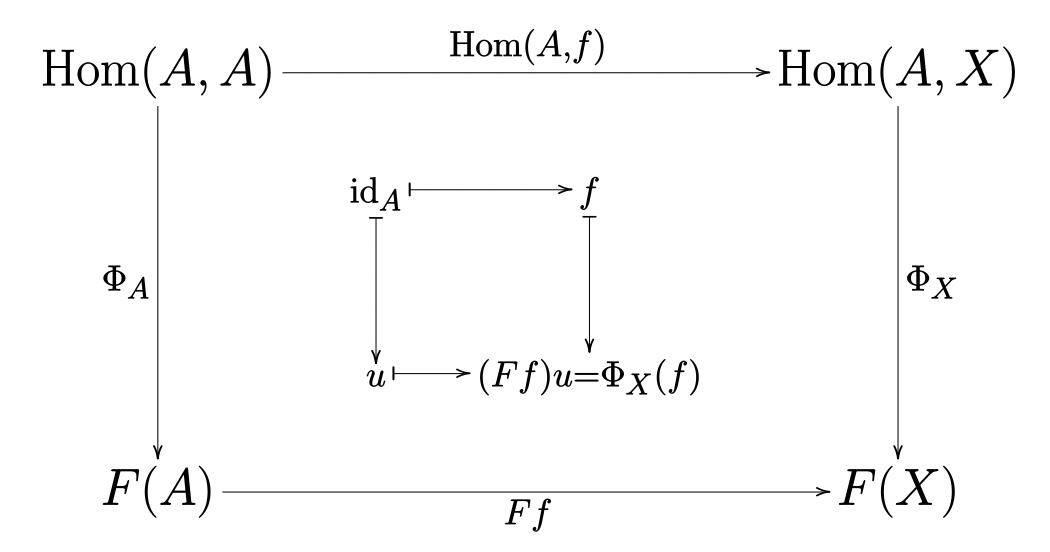
\includegraphics[width=0.75\textwidth]{Yoneda.png}\label{fig:yoneda}
	\end{center}
		\end{figure}
	We notice that this proves injectivity and surjectivity.
	\end{proof}
\begin{exercise}
	Finish the proof of Lemma \ref{lem:Yoneda} by proving naturality. If you need a hint see \cite{Yoneda}.
	\end{exercise}

\begin{defn}
	A \textbf{contravariant functor} $F: \scr{C} \lto \scr{D}$ is an assignment of an object $FC \in \scr{D}$ to every object $C \in \scr{C}$ along with a function for each pair of obejcts $(X,Y)$ in $\scr{C}$
	\begin{equation}
		Ff: \operatorname{Hom}_{\scr{C}}(X, Y) \lto \operatorname{Hom}_{\scr{D}}(FY,FX)
		\end{equation}
	(Note the change of order of $X, Y$), subject to the following conditions:
	\begin{itemize}
		\item For any pair of morphisms $f: X \lto Y, g: Y \lto Z$ in $\scr{C}$ we have $F(g \circ f) = F(f) \circ F(g)$,
		\item For any object $X \in \scr{C}$ we have $F(\operatorname{id}_X) = \operatorname{id}_{FX}$.
		\end{itemize}
	\end{defn}
\begin{exercise}
	Show that the data of a contravariant functor $F: \scr{C} \lto \scr{D}$ is equivalent to the data of a functor $F: \scr{C}^{\operatorname{op}} \lto \scr{D}$.
	\end{exercise}

\begin{exercise}
	Show that there is a ``contravariant" version of Yoneda's Lemma too. That is, prove the following.
	\begin{lemma}
		Let $\scr{C}$ be a small category and $P: \scr{C} \lto \scr{D}$ a contravariant functor. For any object $A \in \scr{C}$ there is a natural bijection
		\begin{align*}
			\operatorname{Nat}(\operatorname{Hom}(\und{0.2}, A), P) \cong P(A)
			\end{align*}
		\end{lemma}
\end{exercise}

In the special case where $P = \operatorname{Hom}(\und{0.2}, B)$ for some object $B \in \scr{C}$, Yoneda's lemma implies the following natural isomorphism.
\begin{equation}
	\operatorname{Nat}(\operatorname{Hom}(\und{0.2}, A), \operatorname{Hom}(\und{0.2}, B)) \cong \operatorname{Hom}(A, B)
	\end{equation}
That is, there is an embedding of categories:
\begin{equation}
	\scr{C} \rightarrowtail \underline{\operatorname{Set}}^{\scr{C}^{\operatorname{op}}}
	\end{equation}
Facts which we will not prove:
\begin{itemize}
	\item $\underline{\operatorname{Set}}^{\scr{C}^{\operatorname{op}}}$ admits all products.
	\item $\underline{\operatorname{Set}}^{\scr{C}^{\operatorname{op}}}$ admits all coproducts.
	\item $\underline{\operatorname{Set}}^{\scr{C}^{\operatorname{op}}}$ admits all limits and colimits.
	\item $\underline{\operatorname{Set}}^{\scr{C}^{\operatorname{op}}}$ admits all exponential objects and a subobject classifier. In fact, $\underline{\operatorname{Set}}^{\scr{C}^{\operatorname{op}}}$ is a \emph{topos}.
	\end{itemize}
All of these holds whether $\scr{C}$ has any of this structure or \emph{none}. In fact, even more can be said, we know what the excess in $\underline{\operatorname{Set}}^{\scr{C}^{\operatorname{op}}}$ is:
\begin{proposition}
	Every object $P \in \underline{\operatorname{Set}}^{\scr{C}^{\operatorname{op}}}$ is a colimit of elements in the image of $\scr{C}$ under the yoneda embedding.
	\end{proposition}
Suggestion: somebody makes a talk out of this.
















\begin{thebibliography}{9}
	\bibitem{Yoneda} W. Troiani, \emph{Course notes for the Séminaire étudiant de théorie des catégorie}, \url{https://williamtroiani.github.io/CategoryTheory/Lecture6.pdf}
	\end{thebibliography}

\end{document}